\subsubsection{\stid{6.03} SNL ATDM Software Technologies}

\paragraph{Overview} \leavevmode \\

The SNL ATDM Software Technologies projects are now aggregated to include Kokkos, Kokkos kernels, VTK-m, and Operating Systems and On-Node Runtime efforts. 

The Kokkos programming model and C++ library enable performance portable on-compute-node parallelism for HPC/exascale C++ applications. Kokkos has been publicly available at http://github.com/kokkos/kokkos since May 2015 and is being used and evaluated by projects at DOE laboratories, PSAAP-II centers, other universities, and organizations such as DoD laboratories. Kokkos library implementation consists of a portable application programmer interface (API) and architecture specific back-ends, including OpenMP, Intel Xeon Phi, and CUDA on NVIDIA GPU. These back-ends are developed and optimized as new application-requested capabilities are added to Kokkos, back-end programming mechanisms evolve, and architectures change.

Kokkos Kernels implements on-node shared memory computational kernels for linear algebra and graph operations, using the Kokkos shared-memory parallel programming model. Kokkos Kernels forms the building blocks of a parallel linear algebra library like Tpetra in Trilinos that uses MPI and threads for parallelism, or it can be used stand-alone in ECP applications. Kokkos Kernels supports several Kokkos backends to support architectures like Intel CPUs, KNLs and NVIDIA GPUs. The algorithms and the implementations of the performance-critical kernels in Kokkos Kernels are chosen carefully to match the features of the architectures. This allows ECP applications to utilize high performance kernels and transfers the burden to Kokkos Kernels developers to maintain them in future architectures. Kokkos Kernels also has support for calling vendor provided libraries where there are optimized kernels available.

VTK-m is a toolkit of scientific visualization algorithms for emerging processor architectures. VTK-m supports the fine-grained concurrency for data analysis and visualization algorithms required to drive extreme scale computing by providing abstract models for data and execution that can be applied to a variety of algorithms across many different processor architectures.  The ECP/VTK-m project is building up the VTK-m codebase with the necessary visualization algorithm implementations that run across the varied hardware platforms to be leveraged at the exascale. We will be working with other ECP projects, such as ALPINE, to integrate the new VTK-m code into production software to enable visualization on our HPC systems.  For the ASC/ATDM program, the VTK-m project will concentrate on support of ATDM applications and ASC’s Advanced Technology Systems (ATS) as well as the ASTRA prototype system at Sandia.  General information about VTK-m as well as source code can be found at: http://m.vtk.org.

The OS and On-Node Runtime project focuses on the design, implementation, and evaluation of operating system and runtime system (OS/R) interfaces, mechanisms, and policies supporting the efficient execution of application codes on next-generation platforms. Priorities in this area include the development of lightweight tasking techniques that integrate network communication, interfaces between the runtime and OS for management of critical resources (including multi-level memory, non-volatile memory, and network interfaces), portable interfaces for managing power and energy, and resource isolation strategies at the operating system level that maintain scalability and performance while providing a more full-featured set of system services. The OS/R technologies developed by this project will be evaluated in the context of ATDM application codes running at large-scale on ASC platforms. Through close collaboration with vendors and the broader community, the intention is to drive the technologies developed by this project into vendor-supported system software stacks and gain wide adoption throughout the HPC community.

\paragraph{Key  Challenges} \leavevmode \\

\subparagraph{Kokkos:} The many-core revolution in computing is characterized by:
(1) a steady increase in the number of cores within individual computer chips;
(2) a corresponding decrease in the amount of memory per core that must be shared by the cores of a chip, and,
(3), the diversity of computer chip architectures.
This diversity is highly disruptive because each architecture imposes different complex
and sometimes conflicting requirements on software to perform well on an architecture.
Application software development teams are confronted with the dual challenges of:
(1) inventing new parallel algorithms for many-core chips,
(2) learning the different programming mechanisms of each architecture, and
(2), creating and maintaining separate versions of their software specialized for each architecture.
These tasks may involve considerable overhead for organizations in terms of time and cost.
Adapting application software to changing HPC requirements is already becoming a large expense for
HPC users and can be expected to grow as the diversity of HPC architectures continues to rise.
An alternative, however, is creating software that is performance portable across current and future architectures.

\subparagraph{Kokkos Kernels:} There are several challenges associated with the Kokkos Kernels work. Part of the complexity arises because profiling tools are not yet full mature for advanced architectures and in this context profiling involves the interplay of several factors which require expert judgment to improve performance.  Another challenging aspect is working on milestones that span a variety of projects and code bases. There is a strong dependence on the various application code development teams for our own team's success. In addition, we face a constant tension between the need for production ready tools and components in a realm where the state-of-the-art is still evolving.

\subparagraph{VTK-m:} The scientific visualization research community has been building scalable HPC algorithms for over 15 years, and today there are multiple production tools that provide excellent scalability \cite{ParaView,Catalyst}. That said, there are technology gaps in data analysis and visualization facing ATDM applications as they move to Exascale.  As we approach Exascale, we find that we can rely less on disk storage systems as a holding area for all data between production (by the simulation) and consumption (by the visualization and analysis). To circumvent this limitation, we must integrate our simulation and visualization into the same workflow and provide tools that allows us to run effectively and capture critical information.

\subparagraph{OS \& ONR:} Exascale challenges for system software span the areas of operating systems, networks, and run time systems.  Container technologies are by now ubiquitous in the cloud computing space, but for High Performance Computing their immense potential has been limited by concerns about compatibility with security models and overhead costs.  As vendors bring forward new network hardware for exascale, both vendors and application programmers lack insight into how applications actually use networks in practice, especially regarding the characteristics of the messages sent in production codes.  As programming models like OpenMP at the node level and MPI at the inter-node level evolve, the particular needs of DOE applications must be addressed in both the development of standards and evaluation of provided run time system implementations.



\paragraph{Solution Strategy} \leavevmode \\

\subparagraph{Kokkos: } The Kokkos team developed a parallel programming model with flexible enough semantics that it can be mapped on a diverse set of HPC architectures including current multi-core CPUs and massively parallel GPUs.
The programming model is implemented using C++ template abstractions, which allow a compile time translation to the underlying programming mechanism on each platform, using their respective primary tool chains.
Compared to approaches which rely on source-to-source translators or special compilers, this way leverages the investment of vendors in their preferred programming mechanism without introducing additional, hard to maintain, tools in the compilation chain.

\begin{figure}[ht!]
\centering
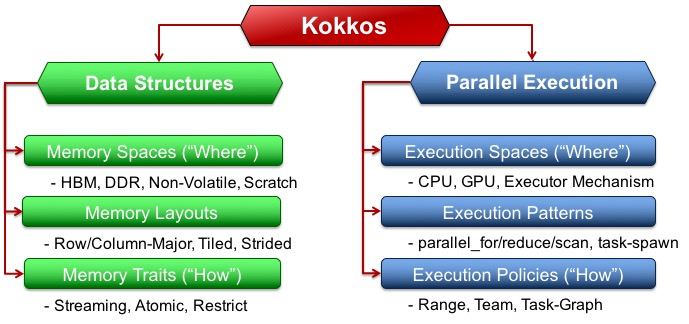
\includegraphics[width=90mm]{projects/2.3.6-NNSA/2.3.6.03-SNL-ATDM/kokkos-abstractions.jpg}
\caption{Kokkos Execution and Memory Abstractions}
\end{figure}

\subparagraph{Kokkos Kernels:} The Kokkos Kernels team is taking a staged approach to profiling in regards to target architectures and the algorithms involved. We are also coordinating on a regular basis with the other projects that are involved in our work to minimize impediments. In response to the need for production ready tools, we are focusing on a hierarchical approach that involves producing robust, hardened code for core algorithms while simultaneous pursuing research ideas where appropriate. 
 
\subparagraph{VTK-m:} The VTK-m team is addressing its challenges through
development of portable visualization algorithms for VTK-m and leveraging and
expanding the Catalyst~\cite{Catalyst}  \emph{in situ} visualization library to
apply this technology to ATDM applications on ASC platforms.  VTK-m uses the
notion of an abstract device adapter, which allows algorithms written once in
VTK-m to run well on many computing architectures.  The device adapter is
constructed from a small but versatile set of data parallel primitives, which
can be optimized for each platform~\cite{Blelloch1990}.  It has been shown that
this approach not only simplifies parallel implementations, but also allows
them to work well across many platforms~\cite{Lo2012,Larsen2015,Moreland2015}.

\subparagraph{OS \& ONR:} The OS \& ONR team is buying down risk for the use of containers by demonstrating exemplar application containerizations, e.g., for the ATDM SPARC application.  We work with facilities staff to develop and implement strategies to deploy containers on our HPC systems and with dev-ops teams to ease the developer burden for code teams seeking to use containers.  To better understand network resource utilization, we use an MPI simulator that accepts real network traces of application executions as inputs and provides detailed analysis to inform network hardware vendors and application developers alike.  We participate actively in both the OpenMP Language Committee and MPI Forum.


%%%%%%%%%%%%%%%%%%%%%%%%%%%%%%%%%%%%%%%%%%%%%%%%%%%

\paragraph{Recent Progress} \leavevmode \\


\subparagraph{Kokkos:}  Kokkos provided a production quality performance portability abstraction to applications and software technology projects under ATDM and ECP which allows them to run on all currently deployed DOE production compute platforms. Support for new platforms was generally in place on the relevant testbeds, before the production machines were delivered.   The development of a number of new features based on customer needs improved the applicability of Kokkos for a wide range of applications. These include abstractions to seamlessly switch between data replication and atomic operation for scatter-add algorithms, improved flexibility of subview, tiled layouts, and multi-dimensional loop abstractions.  Direct help with optimization work for applications, helped identify optimal algorithmic choices as well as improvements in the use of Kokkos.


\subparagraph{Kokkos Kernels:} Kokkos Kernels delivered performance portable kernels for the solve phase of the hypersonic simulations in SPARC. The default solver uses dense linear algebra kernels in Kokkos Kernels. This allows SPARC to achieve portable performance on CPU, Intel KNLs and GPUs. In addition, Kokkos Kernels are the default option for several linear algebra kernels in SNL EMPIRE simulations and the Kokkos Kernels symmetric Gauss-Seidel preconditioner, coloring algorithms are the default solver for the momentum equations in Exawind application. 
 
\subparagraph{VTK-m:} VTK-m 1.4 was released in November 2018, with numerous features and improvements, including ZFP compression, clipping, connected components, particle advection and others.  See the ECP VTK-m report for details.  In addition, the SPARC/Catalyst interface was updated to address some changes to the SPARC code including a change of the SPARC parser to a yaml format for its input.  The team also Integrated and hardened the SPARC/Catalyst interface to make it feasible to merge into the SPARC master branch. The SPARC/Catalyst capability enables in situ capabilities to extract surface data of a re-entry vehicle at scale.  The team also developed a prototype of functional tensor approximation/compression using subsets/slices of Openjet data. These include interpolation onto structured mesh followed by JPEG-like compression, Tucker compression, canonical low-rank functional approximation and functional tensor-train. 

\subparagraph{OS \& ONR:} The OS \& ONR team had a number of recent accomplishments.  The KVM hypervisor was enabled on a Cray XC30 system and application performance studies were conducted to determine the overhead of running in a virtual machine versus the native OS. This is the first demonstration of a virtual cluster on a Cray system.  They enabled the use of the Singularity container system on a Cray system and compared the performance of identical containers running on Cray and Amazon EC2 hardware. They enabled the effective coordination of on-node resources between multiple OS/R environments to evaluate and improve performance isolation capabilities. They extended the LogGOPSim simulator to track MPI resource usage without perturbing applications in order to better understand the impact of MPI matching behavior to guide hardware implementation choices.  They performed a scaling study comparing a containerized version of Nalu with a native version on a CTS-1 platform, which demonstrated that the container can actually reduce runtime while consuming more memory. Made contributions to the ongoing activities of the MPI Forum and the OpenMP Language Committee. Key efforts include: MPI persistent collectives, MPI sessions, MPI finepoints, OpenMP runtime interoperability, and OpenMP multi-level memory management.


\paragraph{Next Steps} \leavevmode \\


\subparagraph{Kokkos: } The Kokkos team is working with the Path Forward vendors to enable support for their architectures.
This notably includes a new backend, called ROCm, for AMD GPUs, which is primarily developed by AMD itself.
Furthermore, improvements on the dynamic task graph execution on GPUs are planned, in order to reduce the task granularity necessary to make effective use for GPUs.

\subparagraph{Kokkos Kernels:} The primary goal in FY20 is to achieve the performance requirements needed to complete the goals of the ATDM L1 milestone. This will focus on improving the performance of the key kernels used by SPARC and EMPIRE. The primary performance goal for supporting SPARC simulations is to improve the kernel efficiency on Volta architecture and MPI communication performance for the solvers on Sierra platform.  The primary performance goal for supporting EMPIRE simulations is to adapt linear algebra kernels to the Volta architecture and achieve the simulation goals of EMPIRE in terms of number of linear solves per second.
 
\subparagraph{VTK-m:} Starting in FY20, the ATDM/VTK-m project will shift from primarily building functionality into the VTK-m toolkit to addressing the needs of other ST projects and ATDM applications. This work will focus on the three key goals of ECP: performance, integration, and quality. We are also exploring the feasibility of using Kokkos libraries to implement the device porting layer. 

\subparagraph{OS \& ONR:} Demonstrate containers on ATS-1 and ATS-2 to support ATDM developer workflows and demonstrate ATDM workloads running on vendor exascale OS/R stacks, evaluate performance and characterize impact of Sandia tech transfer. Refinement of node resource management and runtime with tech transfer to Kokkos and OpenMP and optimize OS/R resource usage for ATDM workloads and demonstrate performance impact. Contribute to the MPI and OpenMP specifications and engage vendors in support of MPI and OpenMP to meet the needs of Kokkos and ATDM apps.
